\section{System overview and specifications}
\label{ch:overview}

\subsection{Architecture}

The system is organized as a closed-loop learning and control pipeline, as shown in \Cref{fig:arch}. The environment provides the current car state and lidar distances. The lidar vector is transformed into a feature vector, normalized and mapped by the SOM to the best matching unit (BMU). This BMU is the discrete state of the Q-table. The policy selects one action from a finite action set, and the simulator applies it to update the vehicle dynamics.

\begin{figure}[H]
    \centering
    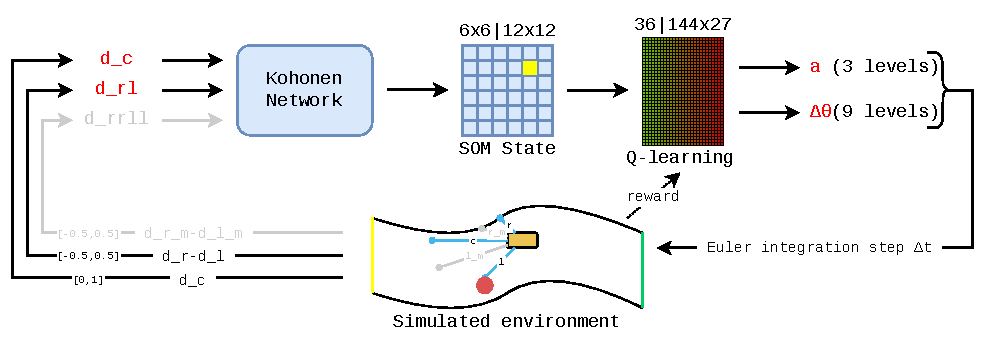
\includegraphics[width=1\textwidth]{images/2/arch.pdf}
    \caption{Block diagram of the implemented perception-control loop}
    \label{fig:arch}
\end{figure}

The workflow consists of five main phases. The track editor creates and modifies JSON tracks. The SOM training script learns the state discretizer from sampled or policy-generated lidar data. The reinforcement learning script trains and checkpoints Q-tables. The inference script loads trained models and runs the policy with a visual interface. The evaluation scripts compute metrics for trained models and produce plots.

\subsection{Environment specification}

Each track is a non-loop circuit described by a centerline, a road width, a start line, a finish line and circular obstacles. The drivable road is obtained by buffering the centerline by half the track width.

The car is represented by a rectangular rigid body. Its kinematic state is
\[
    s_{car} = (x, y, \theta, v),
\]
where $(x,y)$ is the center position, $\theta$ is the heading angle and $v$ is the scalar longitudinal velocity. The default initial pose is the first centerline position for which the full car rectangle lies inside the road, with heading aligned to the local track direction. This prevents the episode from starting in an invalid off-track state.

The final model uses five lidar rays distributed from $-\alpha$ to $+\alpha$, where $\alpha$ is configured as 45 degrees. The three-lidar version has only left, center and right rays.

\subsection{Control specification}

The action space contains 27 actions, defined as the Cartesian product of three acceleration values and nine steering-delta values: in this way, the action space takes into account the dependency of a \textit{good} action from the combination of both acceleration and steering. The acceleration values are full braking, no acceleration and full acceleration. The steering component is a direct heading increment rather than an angular acceleration; this choice was introduced because direct steering was more reactive.
